\begin{center}
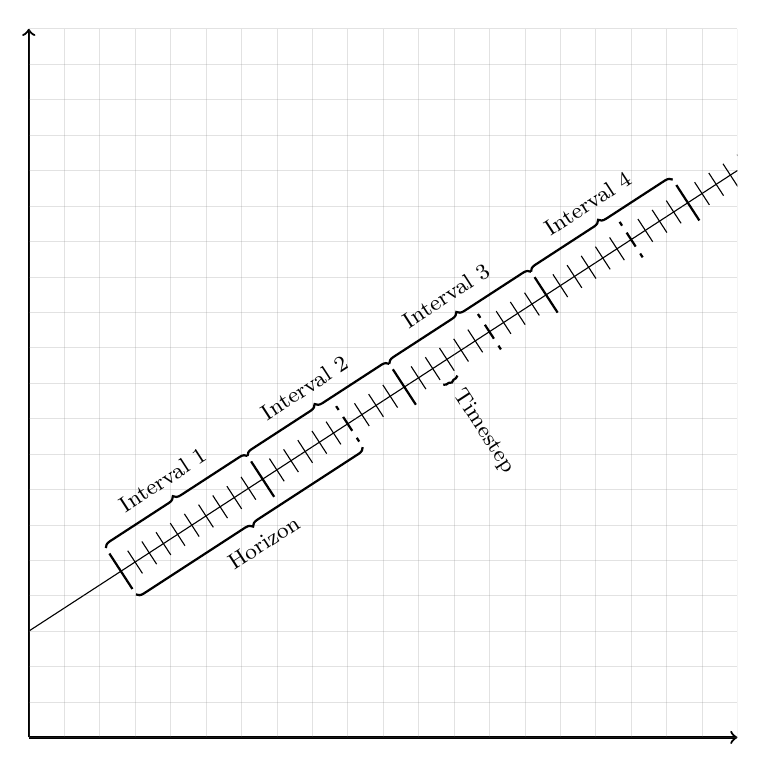
\begin{tikzpicture}
	[scale=0.9,
	axis/.style={->,black,thick}]

	% Draw main axes
	\draw[axis] (0,0) -- (10,0);
	\draw[axis] (0,0) -- (0,10);
	
	\clip (0,0) rectangle (10, 10);
	
	\draw[] (0,1.5) -- (10,8);
	
	% Draw grid
	\foreach \x in {0,0.5,...,10.5}
		\foreach \y in {0,0.5,...,10.5}
		{
			\draw[very thin, gray, opacity=0.01] (\x, 0) -- (\x, 10);
			\draw[very thin, gray, opacity=0.01] (0, \y) -- (10, \y);
		}
	
	\foreach \x/\y in {1.3/2.345, 1.5/2.475, 1.7/2.605, 1.9/2.735, 2.1/2.865, 2.3/2.995,
					   2.5/3.125, 2.7/3.255, 2.9/3.385, 3.1/3.515, 3.3/3.645, 3.5/3.775,
					   3.7/3.905, 3.9/4.035, 4.1/4.165, 4.3/4.295, 4.7/4.555, 4.9/4.685,
					   5.1/4.815, 5.3/4.945, 5.5/5.075, 5.7/5.205, 5.9/5.335, 6.1/5.465,
					   6.3/5.595, 6.7/5.855, 6.9/5.985, 7.1/6.115, 7.3/6.245, 7.5/6.375,
					   7.7/6.505, 7.9/6.635, 8.1/6.765, 8.3/6.895, 8.7/7.155, 8.9/7.285,
					   9.1/7.415, 9.3/7.545, 9.5/7.675, 9.7/7.805, 9.9/7.935, 10.1/8.065}
	{
		\draw[thin] (\x,\y) -- (\x+0.065*1.6, \y-0.1*1.6);
		\draw[thin] (\x,\y) -- (\x-0.065*1.6, \y+0.1*1.6);
	}
	
	\foreach \x/\y in {1.3/2.345, 3.3/3.645, 5.3/4.945, 7.3/6.245, 9.3/7.545}
	{
		\draw[thick] (\x,\y) -- (\x+0.065*2.5, \y-0.1*2.5);
		\draw[thick] (\x,\y) -- (\x-0.065*2.5, \y+0.1*2.5);
	}
	
	\foreach \x/\y in {4.5/4.425, 6.5/5.725, 8.5/7.025}
	{
		\draw[dashed, thick] (\x,\y) -- (\x+0.065*2.5, \y-0.1*2.5);
		\draw[dashed, thick] (\x,\y) -- (\x-0.065*2.5, \y+0.1*2.5);
	}
	
	\draw[thick, decoration={brace, raise=10pt}, decorate]
		(1.3, 2.345) -- (3.3, 3.645) node[midway, above=13pt, sloped] {\footnotesize Interval 1};
		
	\draw[thick, decoration={brace, raise=10pt}, decorate]
		(3.3, 3.645) -- (5.3, 4.945) node[midway, above=13pt, sloped] {\footnotesize Interval 2};
	
	\draw[thick, decoration={brace, raise=10pt}, decorate]
		(5.3, 4.945) -- (7.3, 6.245) node[midway, above=13pt, sloped] {\footnotesize Interval 3};

	\draw[thick, decoration={brace, raise=10pt}, decorate]
		(7.3, 6.245) -- (9.3, 7.545) node[midway, above=13pt, sloped] {\footnotesize Interval 4};
	
	\draw[thick, decoration={brace, mirror, raise=10pt}, decorate]
		(1.3, 2.345) -- (4.5, 4.425) node[midway, below=13pt, sloped] {\footnotesize Horizon};
		
	\draw[thick, decoration={brace, mirror, raise=7pt, amplitude=1}, decorate]
		(5.7, 5.205) -- (5.9, 5.335) node[midway, below=8pt, sloped, rotate=270, anchor=west] {\footnotesize Timestep};

		
		
		
	
\end{tikzpicture}
\end{center}